In this experiment, we test if it is possible to reparametrize curves with piecewise constant and linear SRV form. As test subjects, we interpolate \(r\) and \(q\) given in subsection \ref{subsec:case_1}. The resulting trajectory of the interpolated curves is shown in Figure \ref{fig:curve_1_pc}. Furthermore, by the arguments in section \ref{subsec:discont_curves}, we would not expect a gradient-based optimizer to work in the piecewise constant problem. However, it should work for the continuous problem. As shown in Figure \ref{fig:curve_1_pc_pl_example}, the BFGS algorithm was not able to optimize the cost function corresponding to the piecewise constant interpolated curves. However, the solution to the continuously interpolated problem closely approximated the optimal reparametrization of the original problem. 
\begin{figure}[b]
    \begin{subfigure}[t]{0.5\textwidth}
        \centering
        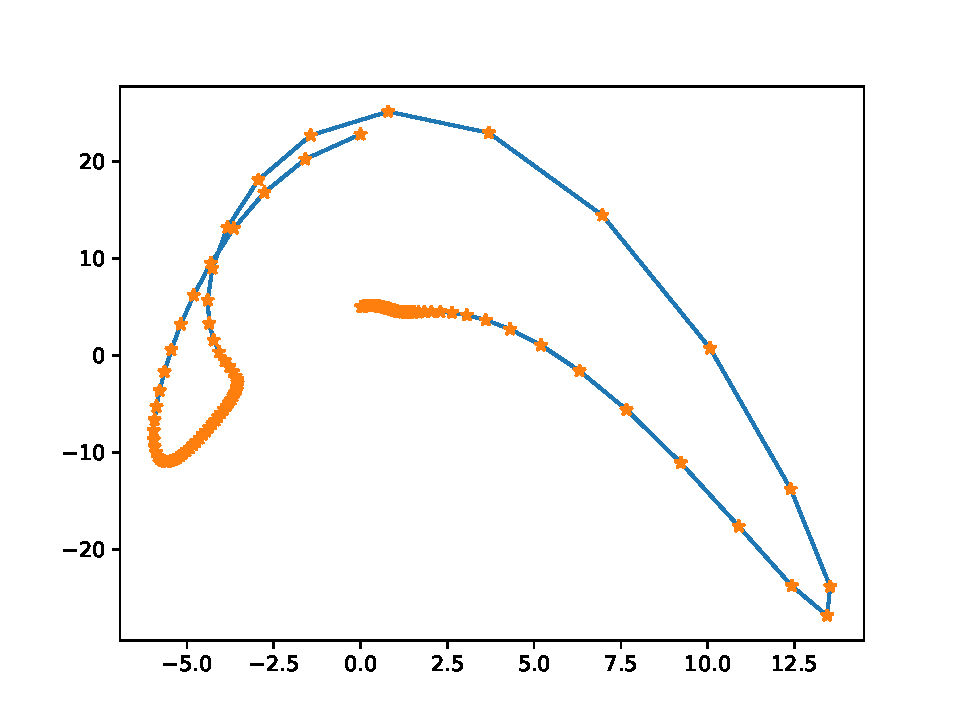
\includegraphics[width=\linewidth]{figures/curve_1_pc/curve_q_pc.pdf}
        \caption{\(\bar q\)}\label{fig:curve_1_pc_q}
    \end{subfigure}
    \begin{subfigure}[t]{0.5\textwidth}
        \centering
        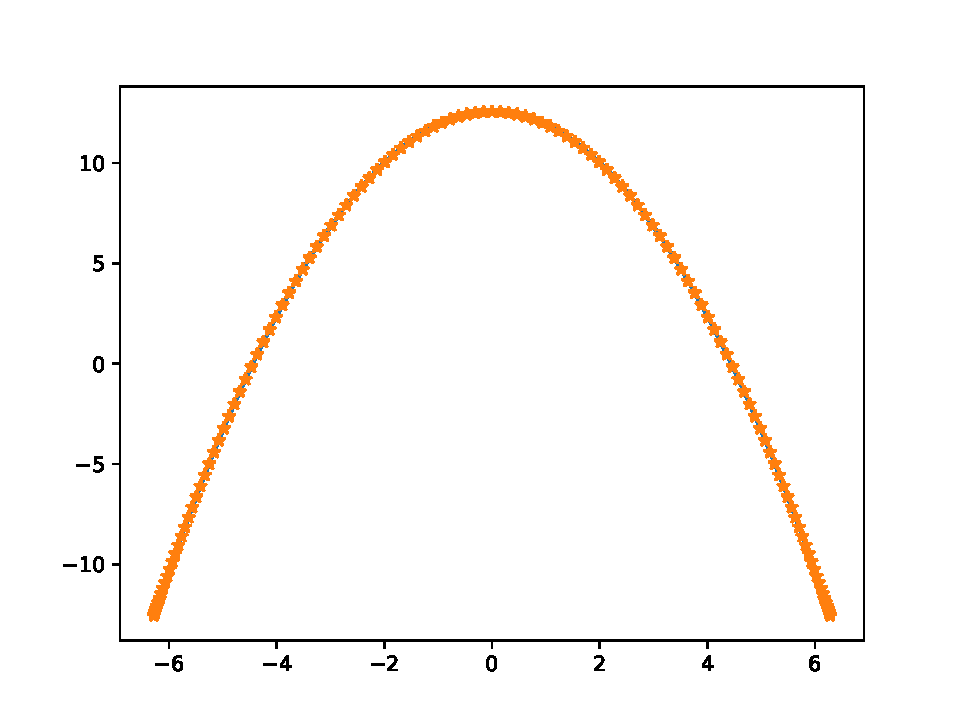
\includegraphics[width=\linewidth]{figures/curve_1_pc/curve_r_pc.pdf}
        \caption{\(\bar r\)}\label{fig:curve_1_pc_r}
    \end{subfigure}
    \caption{The trajectory of \(\bar q\) and \(\bar r\) being piecewise constant interpolations of  \(q\) and  \(r\) from test problem  given in subsection \ref{subsec:case_1}.}\label{fig:curve_1_pc}
\end{figure}

\begin{figure}[t]
    \begin{subfigure}[t]{0.5\textwidth}
        \centering
        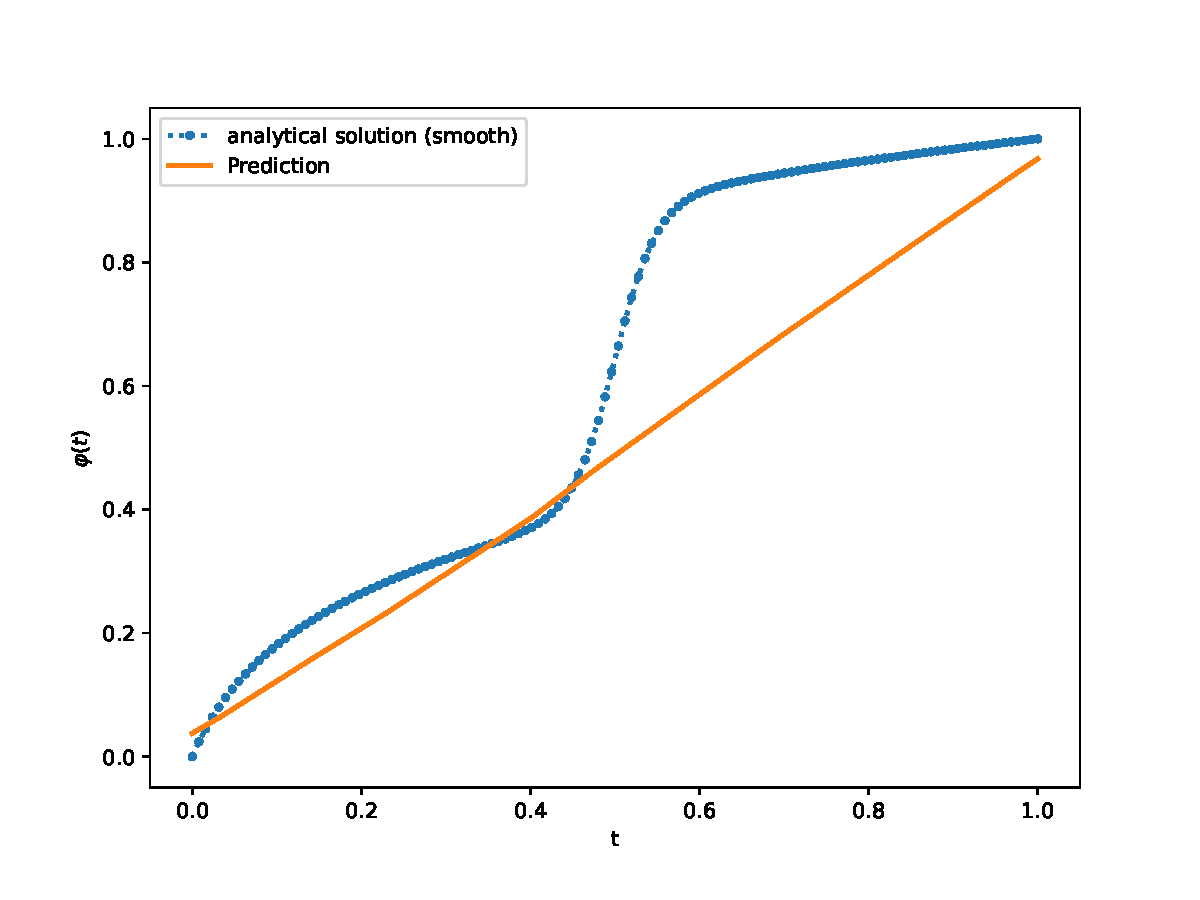
\includegraphics[width=\linewidth]{figures/curve_1_pc/eks_2/plot_0_0.pdf}
        \caption{The approximate optimal reparametrization and analytical solution.}\label{fig:curve_1_pc_solution}
    \end{subfigure}
    \begin{subfigure}[t]{0.5\textwidth}
        \centering
        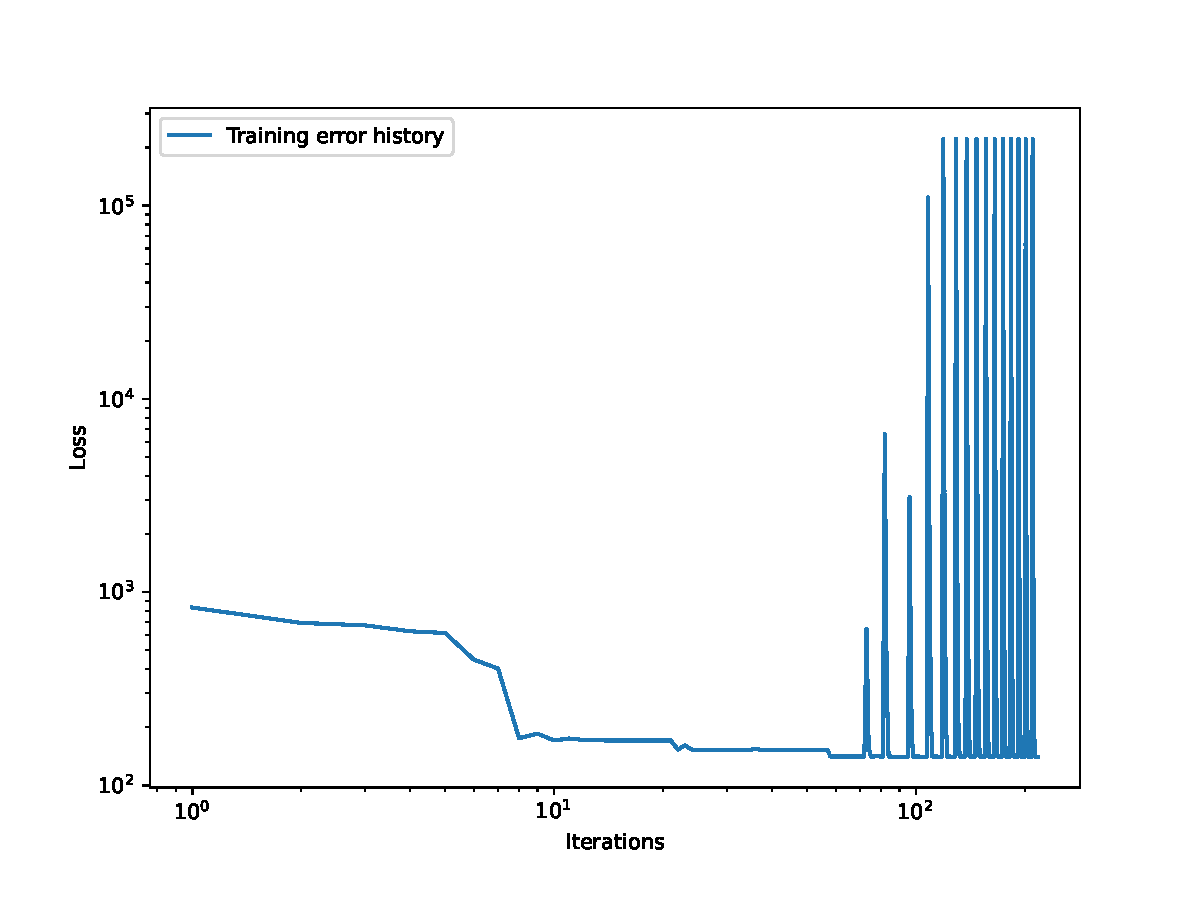
\includegraphics[width=\linewidth]{figures/curve_1_pc/eks_2/history_plot_0.pdf}
        \caption{The cost function \(\mathcal{J}(\theta)\) with each iteration.}\label{fig:curve_1_pc_history}
    \end{subfigure}
    \begin{subfigure}[t]{0.5\textwidth}
        \centering
        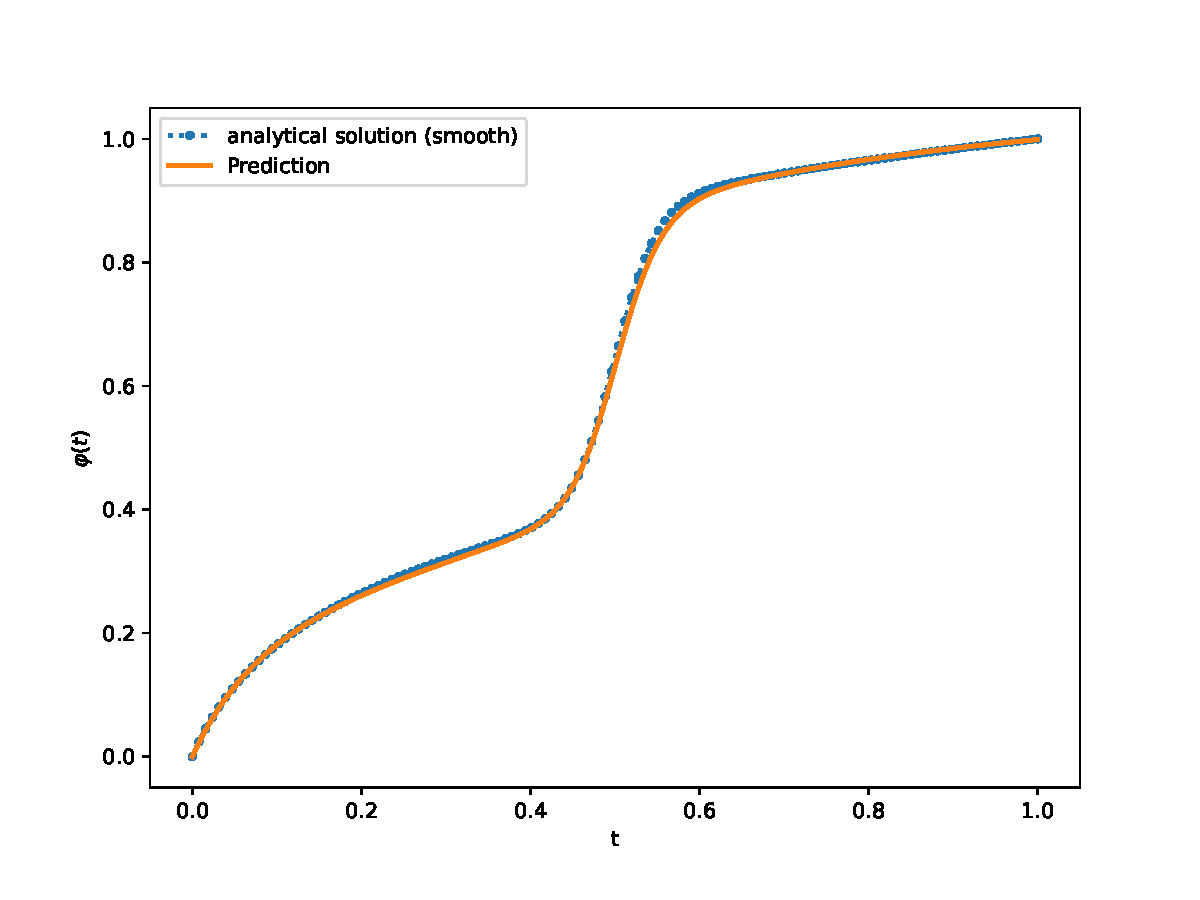
\includegraphics[width=\linewidth]{figures/curve_1_pl/exp_2/plot_0_0.pdf}
        \caption{The approximate optimal reparametrization and analytical solution.}\label{fig:curve_1_pl_solution}\end{subfigure}
    \begin{subfigure}[t]{0.5\textwidth}
        \centering
        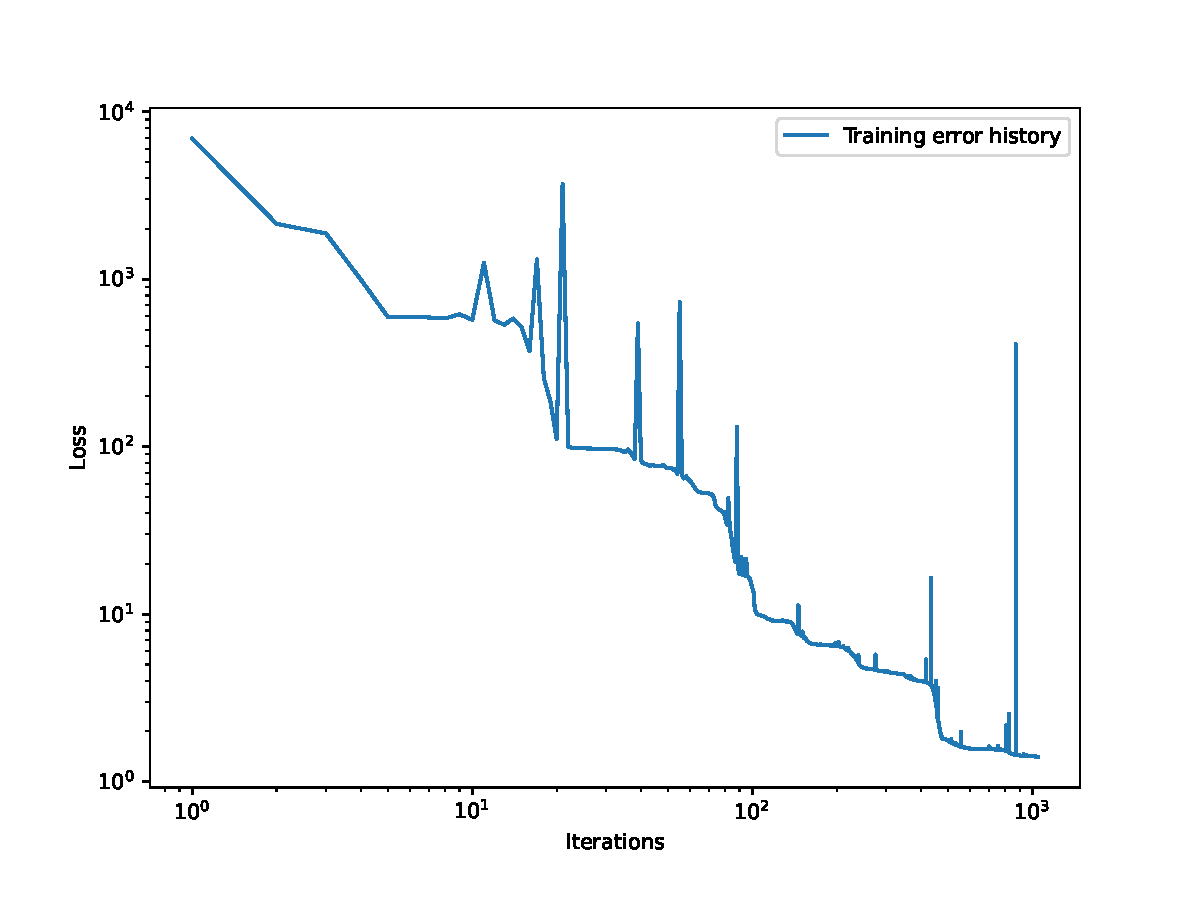
\includegraphics[width=\linewidth]{figures/curve_1_pl/exp_2/history_plot_0.pdf}
        \caption{The cost function \(\mathcal{J}(\theta)\) with each iteration.}\label{fig:curve_1_pl_history}
    \end{subfigure}
    \caption{The approximate solutions to the piecewise constant (\ref{fig:curve_1_pc_solution}) and piecewise linear (\ref{fig:curve_1_pl_solution}) version of test problem from subsection \ref*{subsec:case_1}. The computed reparametrizations are compared to the analytical solution of the original problem, and the corresponding training history is shown in the figure to the right.}\label{fig:curve_1_pc_pl_example}
\end{figure}

\begin{figure}[t]
    \begin{subfigure}[t]{0.5\textwidth}
        \centering
        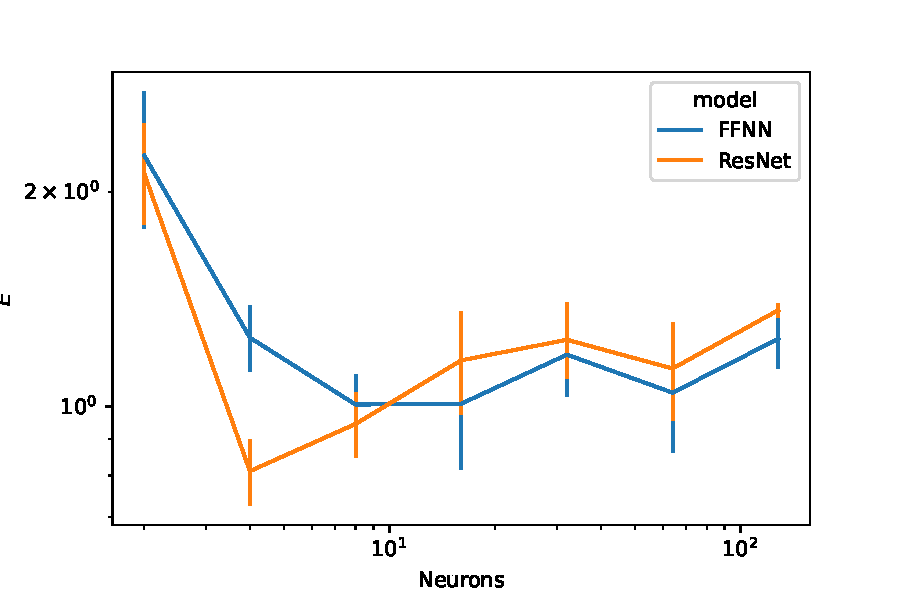
\includegraphics[width=\linewidth]{figures/curve_1_pl/exp_2/neurons_error.pdf}
        \caption{The final cost \(E\) with the number of neurons in each hidden layer.}\label{fig:curve_1_pl_neuron_error}
    \end{subfigure}
    \begin{subfigure}[t]{0.5\textwidth}
        \centering
        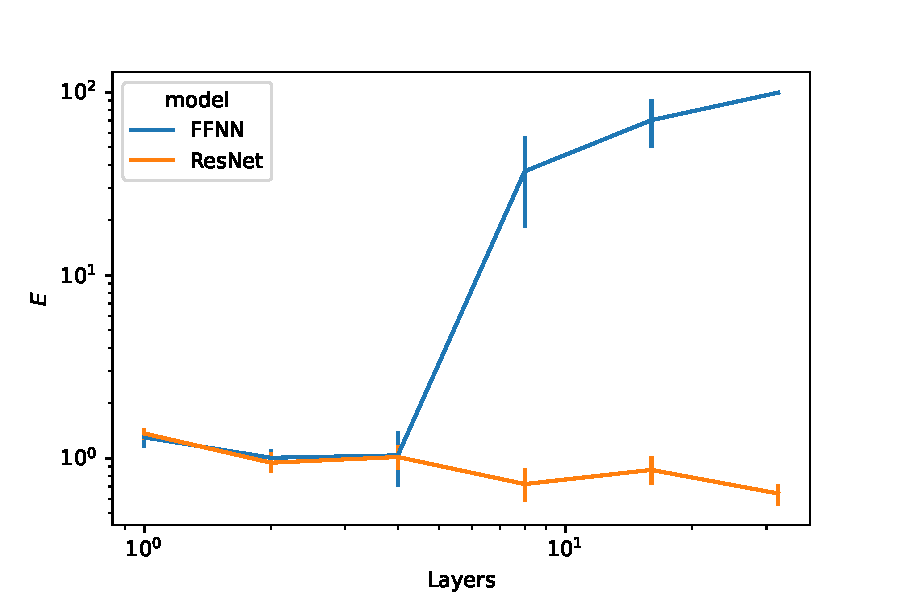
\includegraphics[width=\linewidth]{figures/curve_1_pl/exp_2/layer_error.pdf}
        \caption{Final cost \(E\) with the number of layers.}\label{fig:curve_1_pl_layer_error}
    \end{subfigure}
    \caption{Result of ensemble training for the piecewise linear version of test problem with different number of neurons and hidden layers. In Figure \ref{fig:curve_1_pl_neuron_error} the number of layers was fixed at 2. In Figure \ref{fig:curve_1_pl_layer_error} the number of neurons is fixed at 8 per hidden layer. The error bars denote a 80\% confidence interval found by bootstrapping.}\label{fig:curve_1_pl_eks}
\end{figure}

Since neural reparametrization solved the continuous problem, we also performed ensemble training. The result is shown in Figure \ref{fig:curve_2_layer_error}, where we observe that residual networks outperform fully connected feedforward networks on many layers. 